%%% LaTeX Template: Designer's CV
%%%
%%% Source: http://www.howtotex.com/
%%% Feel free to distribute this template, but please keep the referal to HowToTeX.com.
%%% Date: March 2012


%%%%%%%%%%%%%%%%%%%%%%%%%%%%%%%%%%%%%
% Document properties and packages
%%%%%%%%%%%%%%%%%%%%%%%%%%%%%%%%%%%%%
\documentclass[a4paper,12pt,final]{memoir}

% misc
\renewcommand{\familydefault}{bch}	% font
\pagestyle{empty}					% no pagenumbering
\setlength{\parindent}{0pt}			% no paragraph indentation


% required packages (add your own)
\usepackage{flowfram}										% column layout
\usepackage[top=1cm,left=1cm,right=1cm,bottom=1cm]{geometry}% margins
\usepackage{graphicx}										% figures
\usepackage{url}											% URLs
\usepackage[usenames,dvipsnames]{xcolor}					% color
\usepackage{multicol}										% columns env.
	\setlength{\multicolsep}{0pt}
\usepackage{paralist}										% compact lists
\usepackage{tikz}

%%%%%%%%%%%%%%%%%%%%%%%%%%%%%%%%%%%%%
% Create column layout
%%%%%%%%%%%%%%%%%%%%%%%%%%%%%%%%%%%%%
% define length commands
\setlength{\vcolumnsep}{\baselineskip}
\setlength{\columnsep}{\vcolumnsep}

% frame setup (flowfram package)
% left frame
\newflowframe{0.2\textwidth}{\textheight}{0pt}{0pt}[left]
	\newlength{\LeftMainSep}
	\setlength{\LeftMainSep}{0.2\textwidth}
	\addtolength{\LeftMainSep}{1\columnsep}
 
% small static frame for the vertical line
\newstaticframe{1.5pt}{\textheight}{\LeftMainSep}{0pt}
 
% content of the static frame
\begin{staticcontents}{1}
\hfill
\tikz{%
	\draw[loosely dotted,color=RoyalBlue,line width=1.5pt,yshift=0]
	(0,0) -- (0,\textheight);}%
\hfill\mbox{}
\end{staticcontents}
 
% right frame
\addtolength{\LeftMainSep}{1.5pt}
\addtolength{\LeftMainSep}{1\columnsep}
\newflowframe{0.7\textwidth}{\textheight}{\LeftMainSep}{0pt}[main01]


%%%%%%%%%%%%%%%%%%%%%%%%%%%%%%%%%%%%%
% define macros (for convience)
%%%%%%%%%%%%%%%%%%%%%%%%%%%%%%%%%%%%%
\newcommand{\Sep}{\vspace{1.5em}}
\newcommand{\SmallSep}{\vspace{0.5em}}

\newenvironment{AboutMe}
	{\ignorespaces\textbf{\color{RoyalBlue} About me}}
	{\Sep\ignorespacesafterend}
	
\newcommand{\CVSection}[1]
	{\Large\textbf{#1}\par
	\SmallSep\normalsize\normalfont}

\newcommand{\CVItem}[1]
	{\textbf{\color{RoyalBlue} #1}}


%%%%%%%%%%%%%%%%%%%%%%%%%%%%%%%%%%%%%
% Begin document
%%%%%%%%%%%%%%%%%%%%%%%%%%%%%%%%%%%%%
\begin{document}

% Left frame
%%%%%%%%%%%%%%%%%%%%
\begin{figure}
	\hfill
	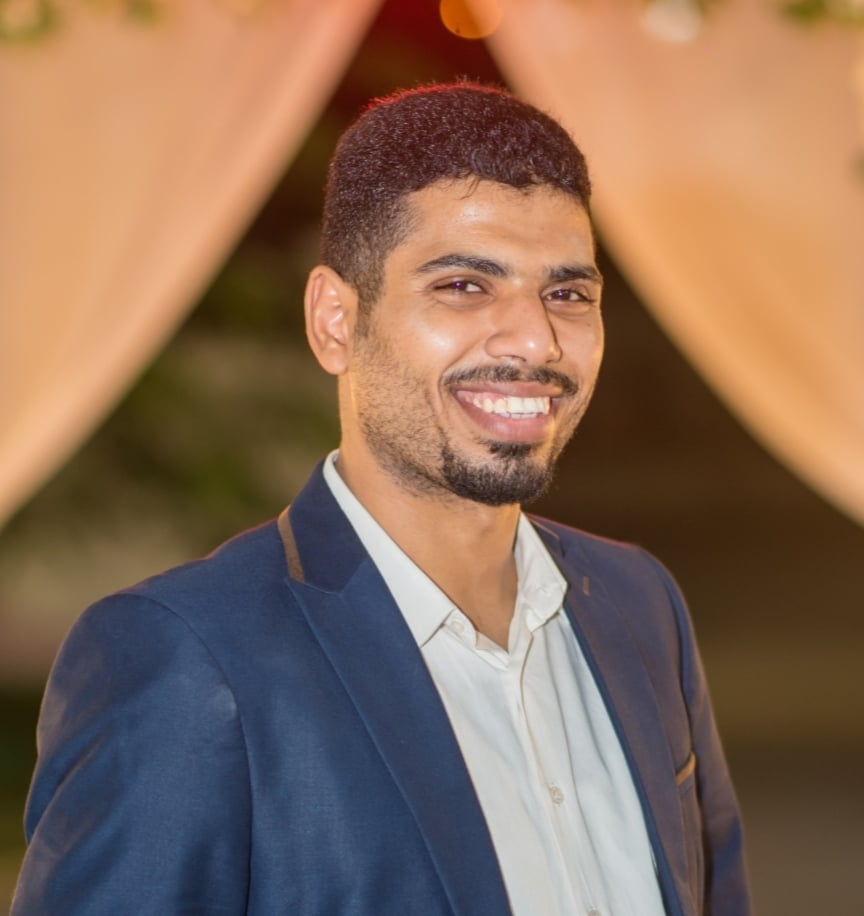
\includegraphics[width=0.6\columnwidth]{shrief.jpg}
	\vspace{-7cm}
\end{figure}

\begin{flushright}\small
	Shrief Abdelazeez \\
	\url{shrief.s.abdelazeez@eng1.cu.edu.eg}  \\
     Tel: 01158159448
\end{flushright}\normalsize
\framebreak


% Right frame
%%%%%%%%%%%%%%%%%%%%
\Huge\bfseries {\color{RoyalBlue} Shrief Abdelazeez} \\
\Large\bfseries  Biomedical Engineer \\

\normalsize\normalfont

% About me
\begin{AboutMe}
I am shrief Sayed Ahmed Abdelazeez. I am graduated from Faculty of Engineering Cairo University, System and Biomedical Engineering Department. I have finished my Premaster Subjects with GPA 4 and now i am preparing my master of science in biomedical engineering. My master thesis is applying deep learning for multi class classification of Whole Slide Images (WSI). I am interested in High performance computing, Data compression, Deep Learning, and Image Processing.
\end{AboutMe}

% Experience
\CVSection{Work Experience}
\CVItem{Jan 2017 - present}\\
\begin{itemize}
  \item RA and Demonstrator at Faculty of Engineering Cairo University.
  \item Senior Calibration Engineer at Medical Equipment Calibration Lab (MECL).
  \item Deep learning course from Udacity using Pytorch.
\end{itemize}
\SmallSep

\CVItem{July 2016 - August 2016, Service Engineer}\\
\begin{itemize}
  \item Service Engineer Trainee at Siemens Company.
  \item Maintenance and installation processes for MRI, CT Equipment.
\end{itemize}
\Sep

\CVItem{Jan 2015 - May 2015, C++ Course}\\
Smart Apps Company
\begin{itemize}
  \item Object Oriented Programming Concepts.
  \item Templates and Standard Template Library (STL).
\end{itemize}
\Sep

\CVItem{Aug 2014 - OCt 2014, C Programming Language Under Linux}\\
Smart Apps Company
\begin{itemize}
\item Working under linux operating environment using c programming language.
\end{itemize}
\Sep

\CVItem{July 2014 - Aug 2014, Service Engineer}\\
Trainee at El Gomhoria Company
\begin{itemize}
  \item Monitors.
  \item Spectrophotometer.
  \item X-ray.
\end{itemize}
\Sep

\clearpage
\framebreak
\framebreak


% Education
\CVSection{Education}
\CVItem{Jan 2019 - present, Master of Science at Biomedical Engineering}\\
Applying Deep learning for Multi class classifications of Whole Slide Images (WSI).
\SmallSep

\CVItem{2017 - 2018, Premaster}\\
\begin{itemize}
  \item Finishing my premaster subjects.
  \item My GPA is 4.
\end{itemize}
\SmallSep

\CVItem{2011 - 2016, Bachelor Degree - System \& Biomedical Engineering}\\
\begin{itemize}
  \item Faculty of Engineering, Cairo University.
  \item Excellent Degree with honor.
  \item Excellent Degree for Graduation Project.
  \item My rank is third of class.
  \item My GPA is 3.9.
\end{itemize}
\Sep

% Skills
\CVSection{Skills}
\CVItem{Programming Skills}
\begin{multicols}{3}
\begin{compactitem}[\color{RoyalBlue}$\circ$]
	\item C/C++ 
	\item Qt Creator
	\item Matlab
	\item MySQL
	\item OpenMP
	\item OpenCL
	\item Python
	\item Pytorch
\end{compactitem}
\end{multicols}
\SmallSep

\CVItem{Computer software Tools}
\begin{multicols}{3}
\begin{compactitem}[\color{RoyalBlue}$\circ$]
	\item Latex
	\item Git 
	\item CMake
	\item \ldots
\end{compactitem}
\end{multicols}
\Sep 




\clearpage
\framebreak
\framebreak

\CVSection{Projects \& Puplications}
\begin{enumerate}
\item \textbf{Graduation Project}:High Performance Distributed Volume Rendering on Heterogenous Platforms.
\item \textbf{Paper in EMBC 2016}:\textit{"Parallel Generation of Digitally Reconstructed Radiographs on Heterogenous Multi-GPU Workstations".}
\item \textbf{Paper ISC 2015}:\textit{"Speaker Recognition Using MFCC and Vector Quatization"}, 2nd best paper.
\end{enumerate}
\Sep

% References
\CVSection{Language Skills}
\begin{enumerate}
\item \textbf{Arabic}: Native Language.
\item \textbf{English}: Good reading, writing, and speaking.
\item \textbf{Deutsch}: Beginner.
\end{enumerate}
\Sep


% References
\CVSection{References}
References upon request.

%%%%%%%%%%%%%%%%%%%%%%%%%%%%%%%%%%%%%
% End document
%%%%%%%%%%%%%%%%%%%%%%%%%%%%%%%%%%%%%
\end{document}